\subsubsection{ClientModel}

\textbf{GoIntentService}
\begin{figure}[H]
	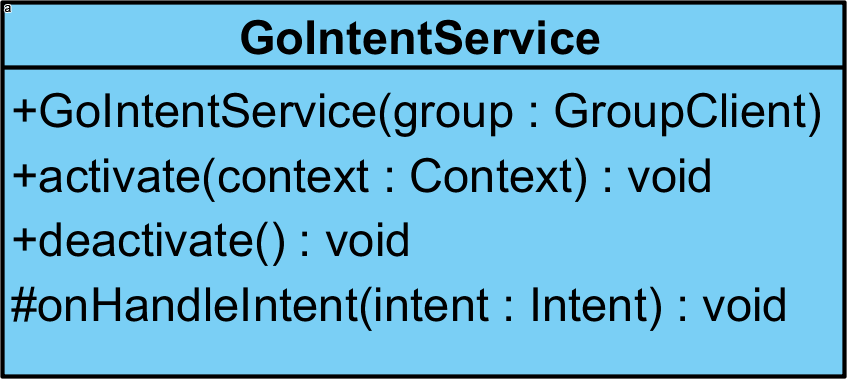
\includegraphics[scale = .3]{res/umlClasses/GoIntentService.png}
	\centering	
\end{figure}
Der GokIntentService kümmert sich um Netzwerkanfragen die den GoStatus, also Anfragen in regelmäßigen Zeitintervallen an den Server sendet und Koordinaten übermittelt. Dieser Service läuft im Hintergrund ab, um die Benutzeroberfläche nicht zu behindern.
\begin{enumerate}
	\item public GoIntentService(group: Group)
		Konstruktor für den IntentService.
	\item public activate(context: Context):void
		GoIntetnService wird aktiviert, wenn der GoStatus aktiviert wurde.
	\item public deactivate():void
		GoIntentService wird deaktiviert, wenn der GoStatus deaktiviert wurde.
	\item protected onHandleIntent(intent: Intent): void
		Für jede Netzwerkanfrage wird ein neuer Thread gestartet und es wird verhindert, dass Anfragen beim Drehen des Bildschirms verloren gehen.
\end{enumerate}

\paragraph{Database}
\begin{figure}[H]
	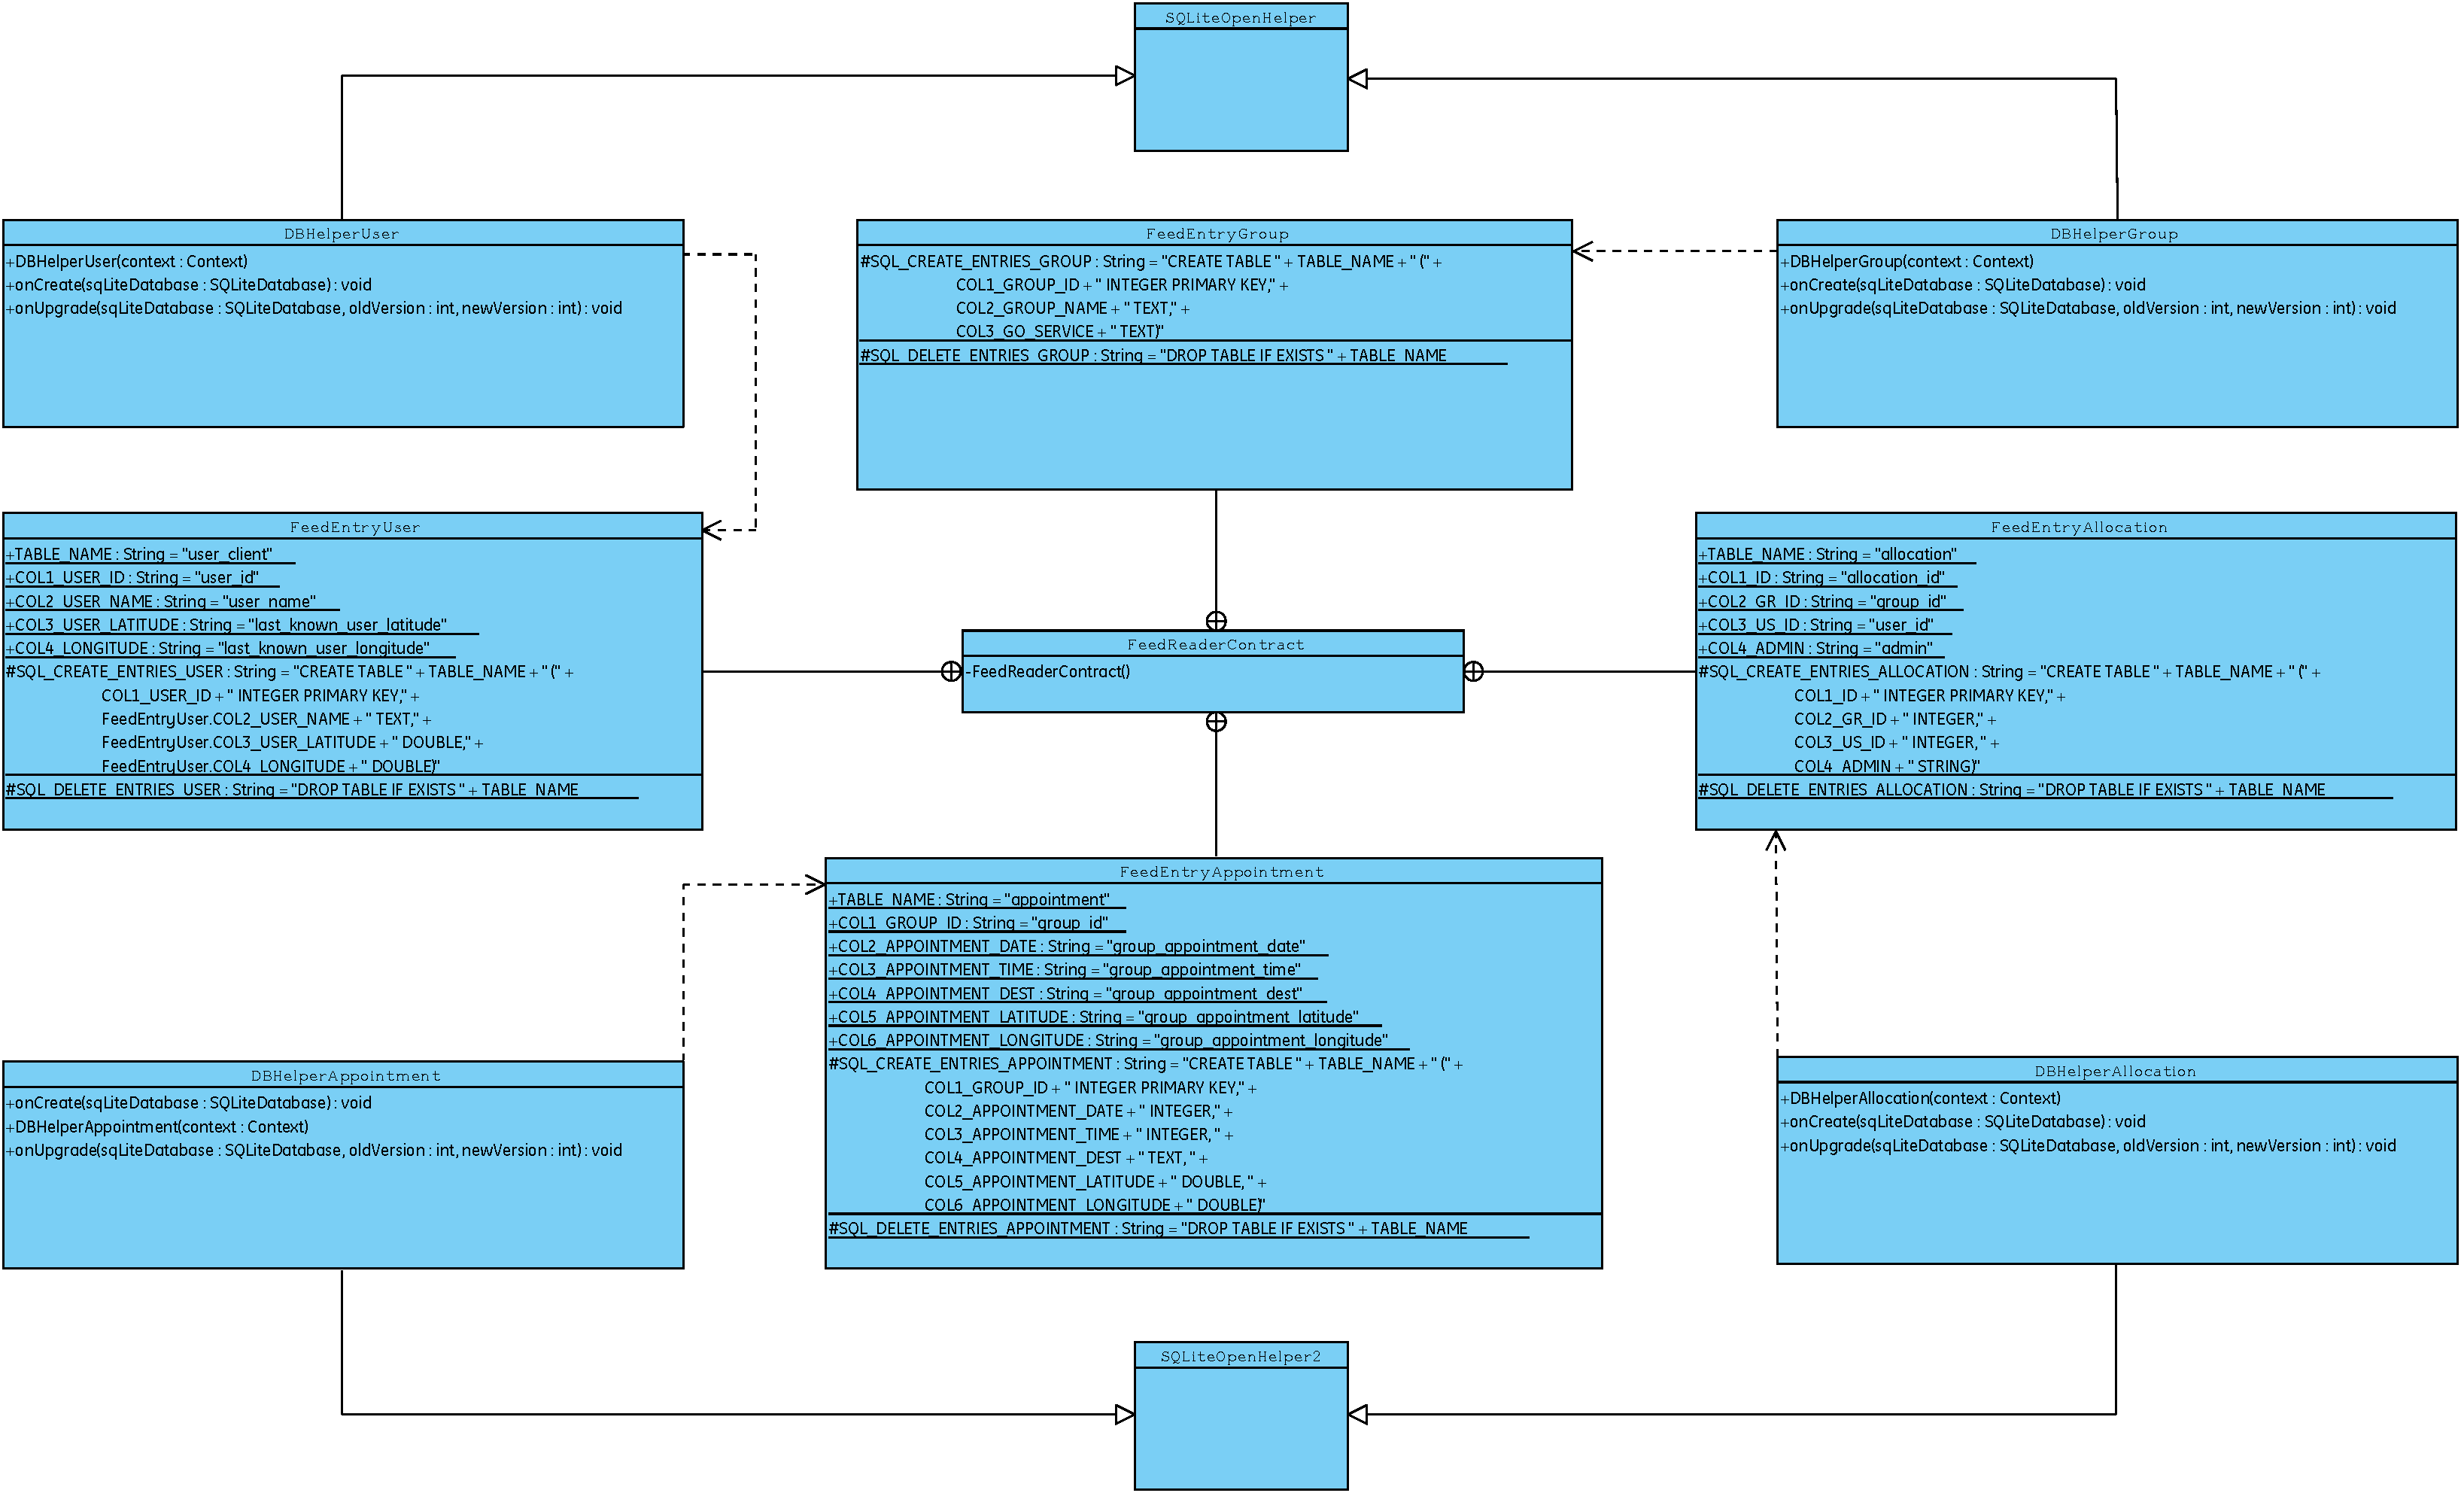
\includegraphics[scale = .3]{res/umlDiagramms/modelClientDatabase.pdf}
	\centering	
\end{figure}

\textbf{DBHelper}\\
Die vier nachfolgenden DBHelper erben ihren Konstruktor und ihre Methoden von SQLiteOpenHelper. 
\begin{enumerate}
	\item public DBHelperGroup(context: Context)\\
		Der Konstruktor definiert dabei den Namen und die Versionsnummer der Datenbank.
	\item public onCreate(sqLiteDatabase: SQLiteDatabase)\\
		Die SQLiteDatenbank wird mit den in FeedReaderEntry definierten Spalten aufgebaut, wenn sie das erste Mal aufgerufen wird.
	\item public onUpgrade(sqLiteDatabase: SQLiteDatabase, oldVersion: int, newVersion: int)\\
		Diese Methode wird verwendet, wenn man die Datenbank verändert hat. Dieser wird dann eine neue Versionsnummer zugeteilt.	
\end{enumerate}
\begin{figure}[H]
	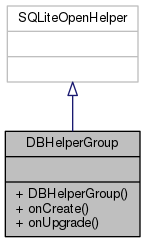
\includegraphics[scale = .5]{res/umlClasses/DBHelperGroup.png}
	\centering	
\end{figure}

\begin{figure}[H]
	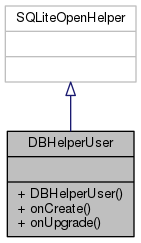
\includegraphics[scale = .5]{res/umlClasses/DBHelperUser.png}
	\centering
\end{figure}

\begin{figure}[H]
	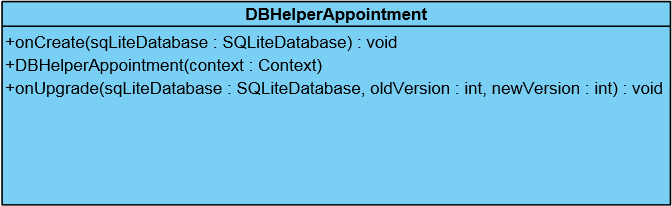
\includegraphics[scale = .58]{res/umlClasses/DBHelperAppointment.png}
	\centering
\end{figure}

\begin{figure}[H]
	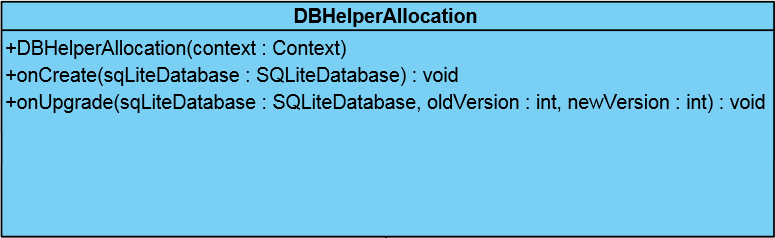
\includegraphics[scale = .5]{res/umlClasses/DBHelperAllocation.png}
	\centering
\end{figure}


\textbf{FeedReaderContract}
\begin{figure}[H]
	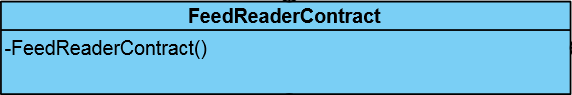
\includegraphics[scale = .5]{res/umlClasses/FeedReaderContract.png}
	\centering
\end{figure}
Die FeedReaderContract Klasse definiert in statischen Innenklassen wie die Tabellen der Datenbank aufgebaut sind. Jede der nachfolgenden FeedEntry Klassen implementiert dabei das Interface BaseColumns.

\begin{enumerate}
	\item public static final CREATE ENTRIES:String\\
		Legt die Spalten wenn die Tabelle generiert wird in genau dieser Reihenfolge an.
	\item public static final DELETE ENTRIES:Strning\\
		Löscht die zuvor definierten Spalteneinträge.
\end{enumerate}

\textbf{FeedEntyGroup}
\begin{figure}[H]
	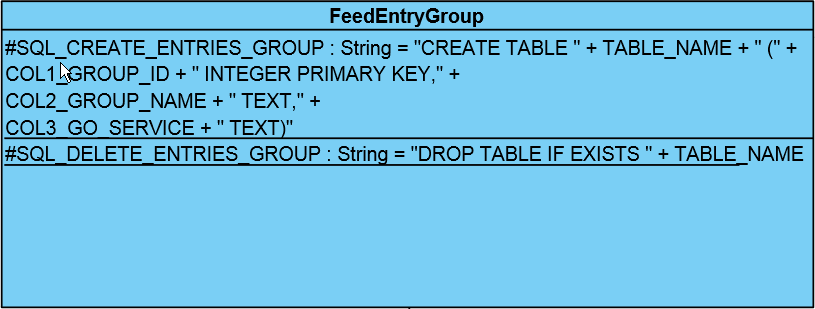
\includegraphics[scale = .5]{res/umlClasses/FeedEntryGroup.png}
	\centering
\end{figure}
Die Innenklasse FeedEntryGroup definiert den Namen und die Spalten der Tabelle, welche die Gruppen auf dem Client speichert. 
Dabei steht in der ersten Spalte die eindeutige Gruppen ID (welche die Zeilen eindeutig unterscheidbar macht), in der zweiten Spalte der eindeutige Gruppenname und in der dritten Spalte, ob der GoService des aktuellen Benutzers für diese Gruppe aktiviert oder deaktiviert ist.
Wenn eine Gruppe gelöscht wird, dann wird auch ihr Eintrag in der Datenbank gelöscht.

\textbf{FeedEntyUser}
\begin{figure}[H]
	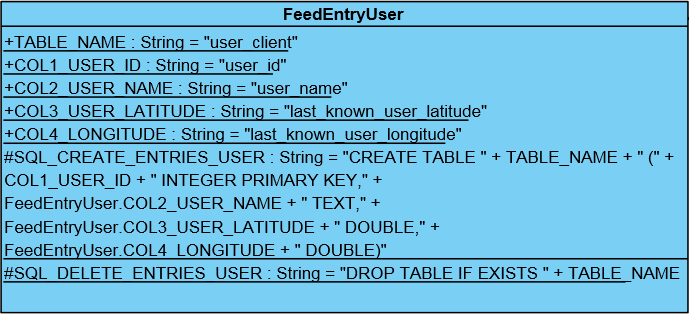
\includegraphics[scale = .6]{res/umlClasses/FeedEntryUser.png}
	\centering
\end{figure}
Die Innenklasse FeedEntryUser definiert den Namen und die Spalten der Tabelle, welche die Benutzer auf dem Client speichert. 
Dabei steht in der ersten Spalte die eindeutige Benutzer ID (welche die Zeilen eindeutig unterscheidbar macht), in der zweiten Spalte der Benutzername und in der dritten und vierten Spalte steht je ein Wert der zuletzt bekannten Gps Daten des jeweiligen Nutzers. 
Es werden nur Benutzer gespeichert mit denen der aktuelle Benutzer in mindestens einer gemeinsamen Gruppe ist.

\textbf{FeedEntyAppointment}
\begin{figure}[H]
	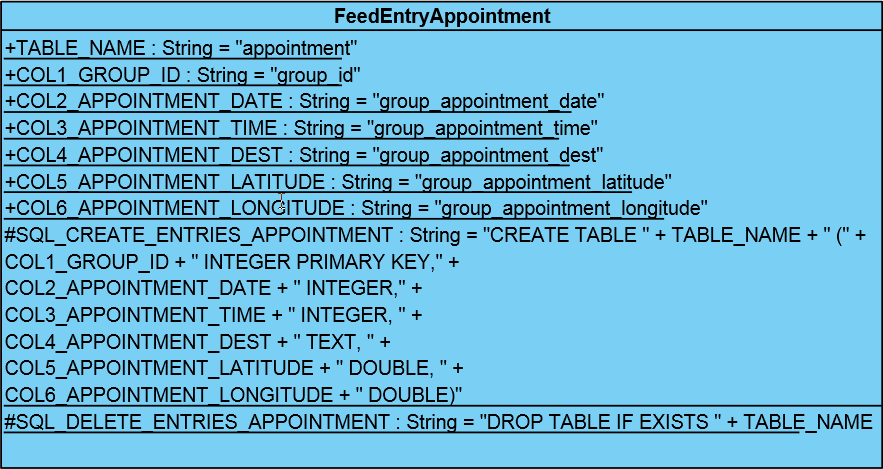
\includegraphics[scale = .5]{res/umlClasses/FeedEntryAppointment.png}
	\centering
\end{figure}
Die Innenklasse FeedEntryAppointment definiert den Namen und die Spalten der Tabelle, welche die Treffpunkte zu jeder Gruppe speichert. Jede Gruppe hat dabei nur eine Zeile, welche den Treffpunkt definiert. 
Dabei steht in der ersten Spalte die Gruppen id (welche die Zeilen eindeutig unterscheidbar macht), in der zweiten Spalte steht das Datum und in der dritten die Uhrzeit des Treffpunktes. In der vierten Spalte steht der Name des Zielortes und in der fünften und sechsten steht jeweils ein Wert der Gps Daten des Zielortes. 
Wenn sich der Treffpunkt der Gruppe ändert, dann werden die Werte des alten Treffpunktes überschrieben.
Sollte die die Gruppe des dazugehörigen Treffpunktes gelöscht werden, dann wird auch der Eintrag in dieser Tabelle gelöscht.

\textbf{FeedEntyAllocation}
\begin{figure}[H]
	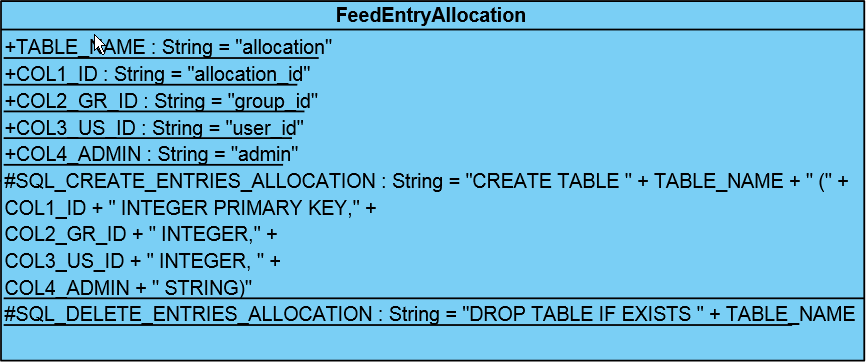
\includegraphics[scale = .5]{res/umlClasses/FeedEntryAllocation.png}
	\centering
\end{figure}
Die Innenklasse FeedEntryAllocation definiert den Namen und die Spalten der Tabelle, welche die jeweiligen Mitglieder jeder Gruppe speichert, in der der aktuelle Benutzer Mitglied ist. Zu jedem Mitglied wird vermerkt, ob dieses Administratorrechte hat.
Dabei steht in der ersten Spalte die Allocation id (welche die Zeilen eindeutig unterscheidbar macht und automatisch hochgezählt), in der zweiten Spalte steht die Gruppen id, in der dritten Spalte die Benutzer id und in der vierten Spalte, ob dieser Benutzer Gruppenadministrator ist oder nicht. 
Gruppen id wird für jedes Gruppenmitglied vermerkt, also kommt mehrmals vor, sobald mehr als ein Benutzer Mitglied dieser Gruppe ist.


\paragraph{ObjectStructure}

\begin{figure}[H]
	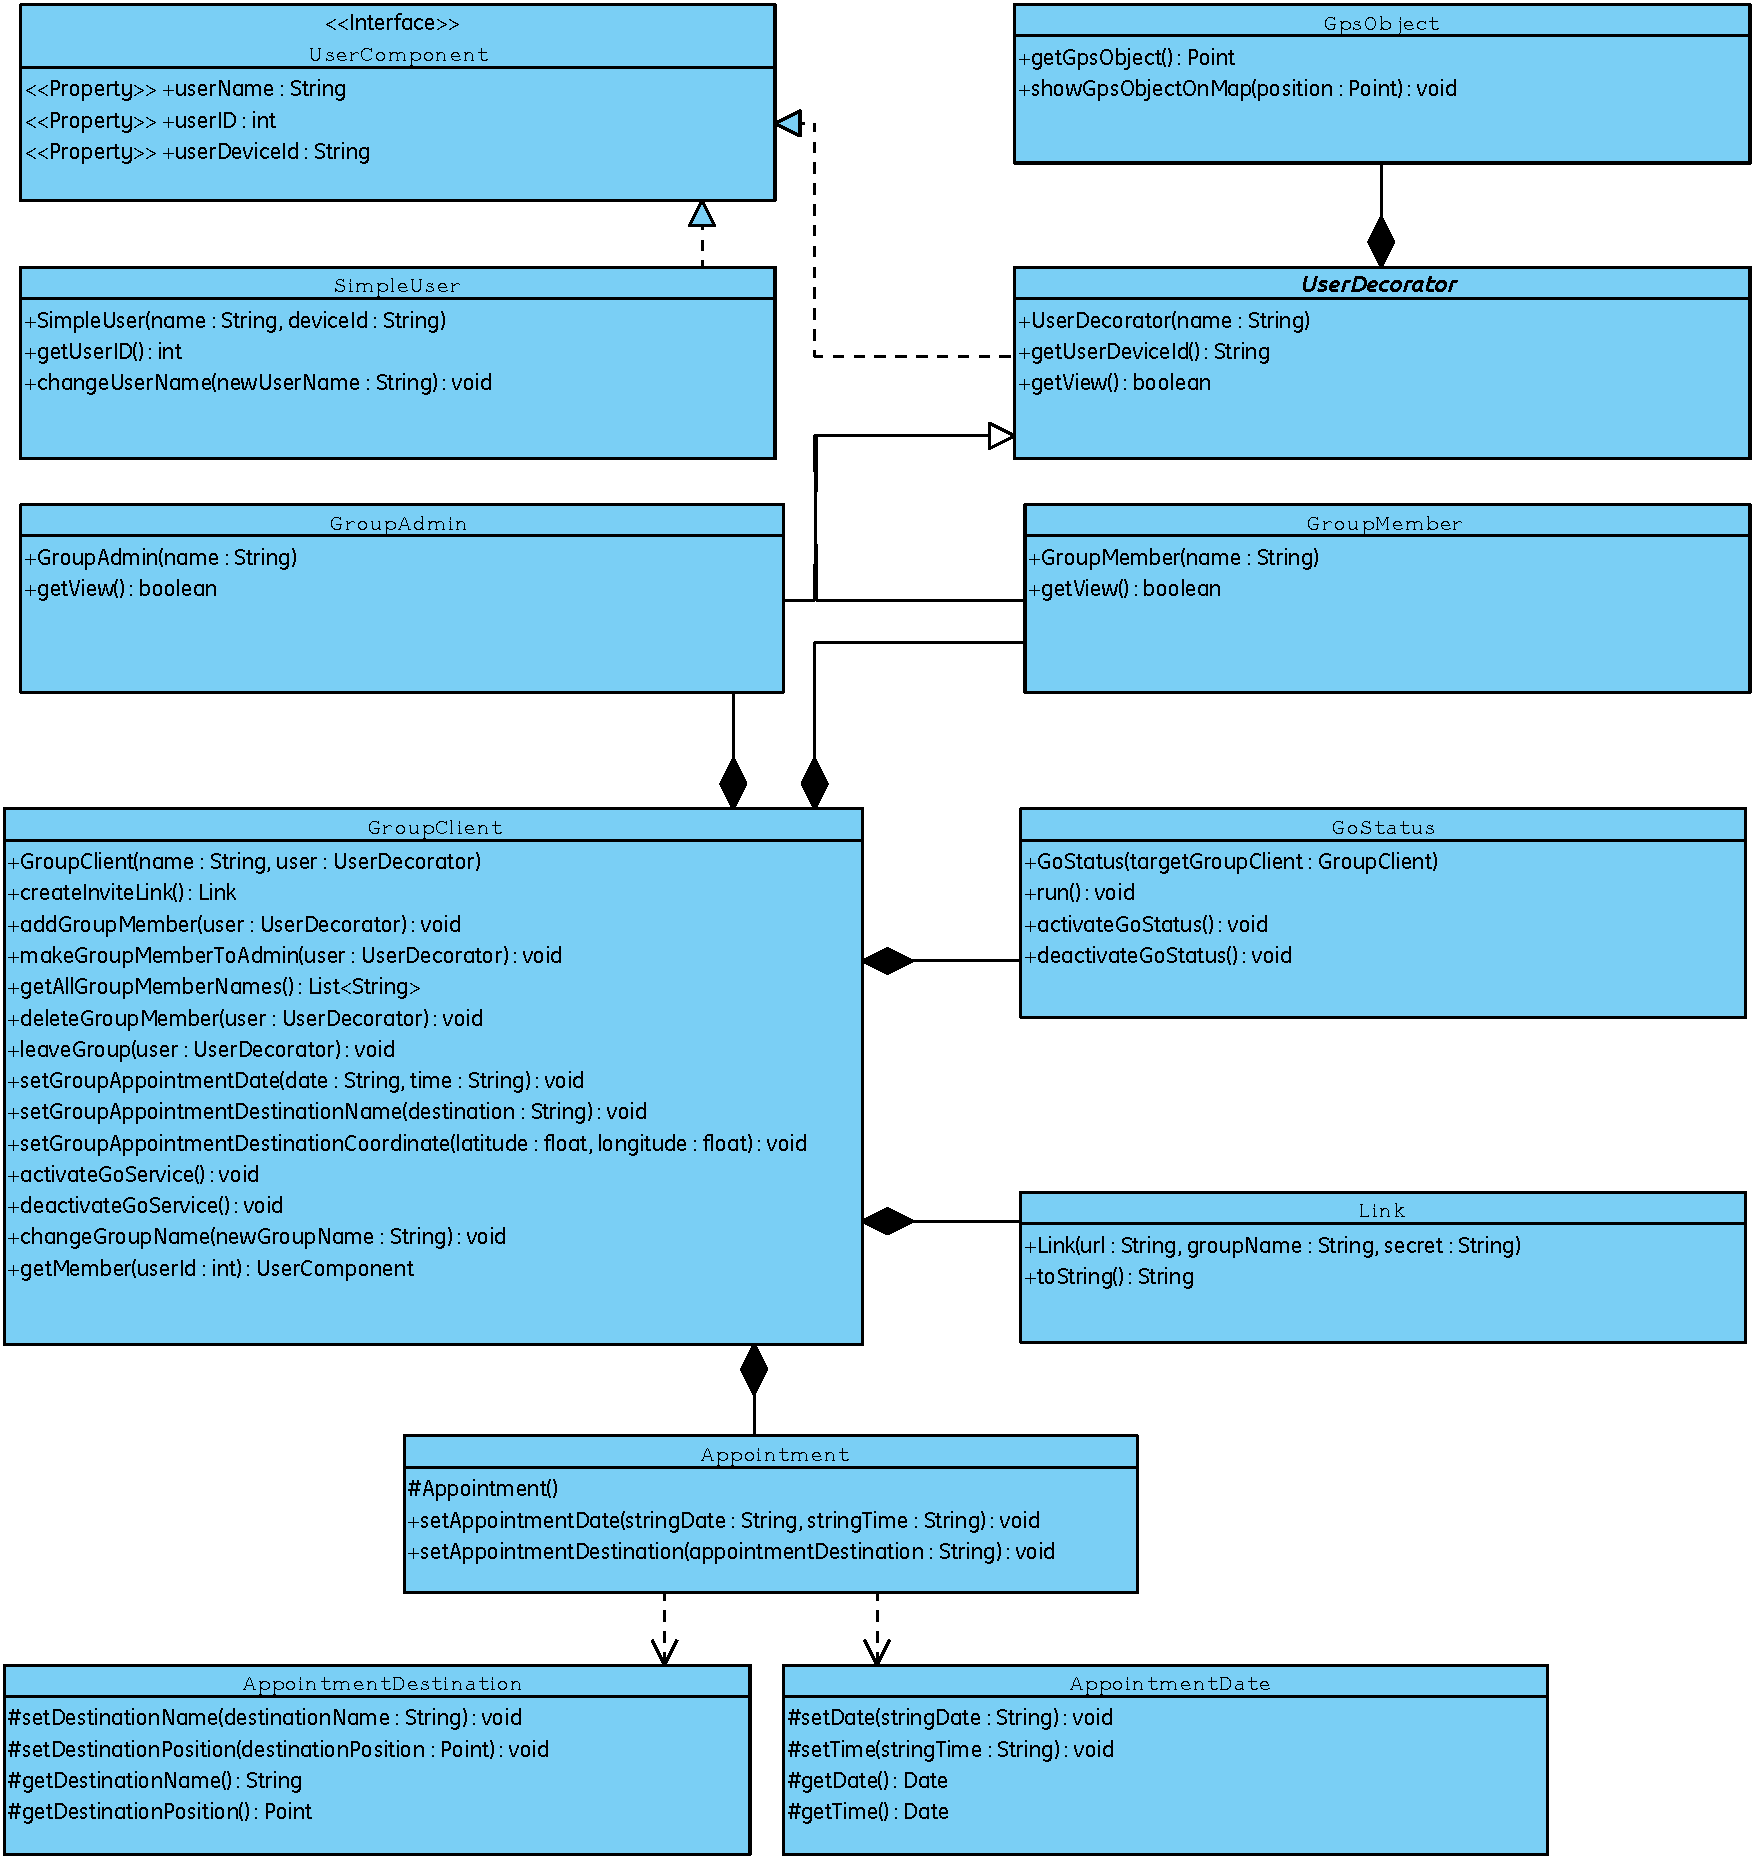
\includegraphics[scale = .5]{res/umlDiagramms/modelClientObjectStructure.pdf}
	\centering	
\end{figure}

\textbf{GroupClient}
\begin{figure}[H]
	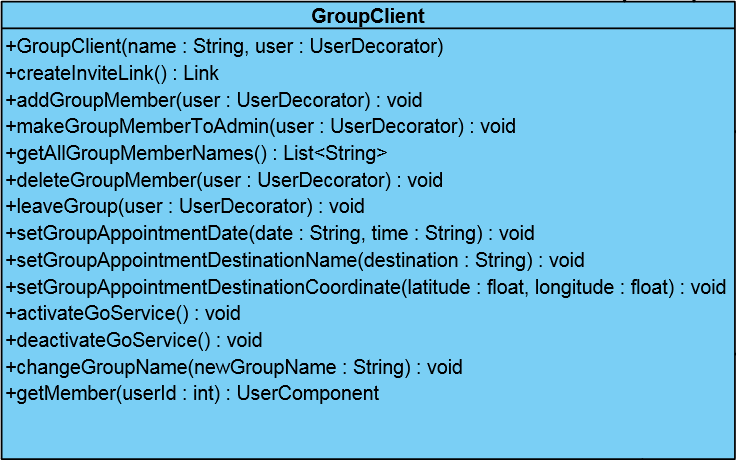
\includegraphics[scale = .5]{res/umlClasses/GroupClient.png}
	\centering
\end{figure}
Die Klasse GroupClient definiert wie eine Gruppe auf dem Client aufgebaut ist und welche Funktionalität ihr zur Verfügung steht.
\begin{enumerate}
	\item public GroupClient(name: String, user: UserDecorator)\\
		Konstruktor der einer neuen Gruppe einen eindeutigen Gruppennamen zuweist und den Ersteller als Gruppenadministrator festlegt.
	\item public createInviteLink():Link\\
		Um ein Gruppenmitglied hinzuzufügen, muss dieses über einen eindeutigen Link beitreten. Wird der Link ausgeführt wird man entweder zu GoApp weitergeleitet (hat App bereits installiert) oder wird dazu aufgefordert diese zu installieren. Der Link ist nicht mehr gültig sobald das Mitglied hinzugefügt wurde. Man muss Administrator sein um diese Funktion verwenden zu können.
	\item public addGroupMember(user: UserDecorator)\\
		Ein Mitglied wird der Gruppe hinzugefügt.
	\item public makeGroupMemberToAdmin(user: UserDecorator)\\
		Ein Gruppenmitglied wird vom Administrator zum Gruppenadministrator gemacht.
	\item public getAllGroupMemberNames():List<String>\\
		Alle Namen der Mitglieder einer Gruppe werden zurückgegeben.
	\item public deleteGroupMember(user:UserDecorator)\\
		Ein Gruppenmitglied wird aus der Gruppe durch den Administrator entfernt.
	\item public leaveGroup(user:UserDecorator)\\
		Ein Mitglied verlässt die Gruppe.
	\item public activateGoService()\\
		Der aktuelle Benutzer aktiviert seinen GoStatus und übermittelt seine GPS Daten an die Gruppe (GPS muss eingeschalten sein).
	\item public deactivateGoService()\\
		Der aktuelle Benutzer deaktiviert seinen GoStatus und wird nicht mehr verfolgt.
	\item public changeGroupName(newGroupName:String)\\
		Der Gruppenadministrator benennt die Gruppe zu einem anderen eindeutigen Namen um.
	\item public getGroupID():int \\
		Die Gruppen Id wird zurückgegeben
	\item public getGroupName():String\\
		Der Gruppenname wird zurückgegeben 
	\item public getGoStatus():GoStatus \\
		Der GoStatus wird zurückgegeben
	\item public getAppointment():Appointment \\
		Das Appointment wird zurückgegeben
	\item public getMember(userId: int):UserComponent \\
		Der Typ des aktuellen Benutzers einer Gruppe (Gruppenmitglied oder Administrator)wird zurückgegeben, um die Ansicht der Gruppe auf seine ihm zugänglichen Funktionen zu beschränken/ erweitern.
\end{enumerate}

\textbf{UserComponent}
\begin{figure}[H]
	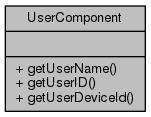
\includegraphics[scale = .5]{res/umlClasses/UserComponent.png}
	\centering
\end{figure}
Dieses Interface ist die erste Komponente des Decorator pattern und definiert grundlegende Funktionen des Benutzers die jederzeit aufgerufen werden können. 

Mit getUserId() kann der Benutzer von anderen Gruppenmitgliedern unterschieden werden, da der Benutzername nicht eindeutig sein muss, die Id aber schon.
Mit getUserDeviceId() kann der Benutzer auf dem Server angelegt werden. Jede Gerätenummer kann nur einmal auf dem Server vorkommen, um Missbrauch der GoApp vorzubeugen.
\begin{enumerate}
	\item public getUserName():String\\
		Benutzername des aktuellen Benutzers kann in der GoApp visualisiert werden.
	\item public getUserID():int\\
		Mit der Benutzer Id kann sich der aktuelle Benutzer unter den anderen Gruppenmitglieder identifizieren.
	\item public getUserDeviceID():String\\
		Die Device Id wird auf dem Server zusammen mit den anderen zwei Werten gespeichert, um einem Endgerät nur einen Benutzer zu erlauben, um Missbrauch zu vermeiden.
\end{enumerate}

\textbf{SimpleUser}
\begin{figure}[H]
	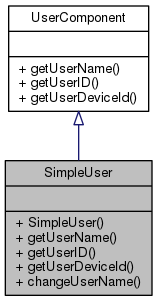
\includegraphics[scale = .5]{res/umlClasses/SimpleUser.png}
	\centering
\end{figure}
Die SimpleUser Klasse implementiert das UserComponent Interface. Der Benutzer ist ein SimpleUser Objekt, wenn er nicht in der Gruppenansicht ist und so weder einem Gruppenadministrator noch einem Gruppenmitglied entspricht.
\begin{enumerate}
	\item public getUserName():String\\
		Siehe UserComponent.
	\item public getUserID():int\\
		Siehe UserComponent.
	\item public getUserDeviceID():String\\
		Siehe UserComponent.
	\item public changeUserName(newUserName: String)\\
	Der aktuelle Benutzer kann seinen Benutzernamen nachträglich ändern.
\end{enumerate}

\textbf{UserDecorator}
\begin{figure}[H]
	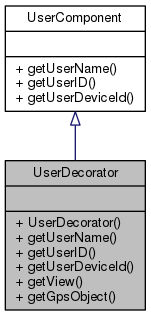
\includegraphics[scale = .5]{res/umlClasses/UserDecorator.png}
	\centering
\end{figure}
Die UserDecorator Klasse ist eine abstrakte Klasse, die wie SimpleUser das UserComponent Interface implementiert. 
\begin{enumerate}
	\item public getUserName():String\\
		Siehe UserComponent.
	\item public getUserID():int\\
		Siehe UserComponent.
	\item public getUserDeviceID():String\\
		Siehe UserComponent.
	\item public getView():boolean\\
		Mit dieser Methode wird bestimmt welche Gruppenansicht der aktuelle Benutzer sieht (die für ein Gruppenmitglied oder die für einen Gruppenadministrator mit zusätzlichen Funktionen).
	\item public getGpsObject():GpsObject\\
		Die Gps Daten des aktuellen Benutzers werden zurück gegeben.
\end{enumerate}

\textbf{GroupAdmin}
\begin{figure}[H]
	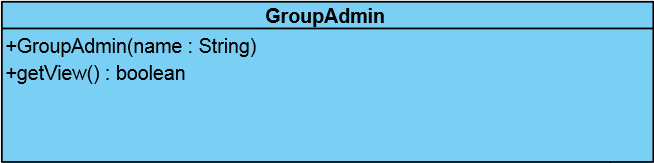
\includegraphics[scale = .5]{res/umlClasses/GroupAdmin.png}
	\centering
\end{figure}
Der Gruppenadministrator unterscheidet sich vom Gruppenmitglied in sofern, dass ihm weitaus mehr Funktionen zur Verfügung stehen, wie Mitglieder hinzufügen/ entfernen und Treffpunkte festlegen.
\begin{enumerate}
	\item public GroupAdmin(name: String)\\
		Konstruktor für einen Gruppenadministrator.
	\item public getView():boolean\\
		Siehe UserDecorator.
\end{enumerate}

\textbf{GroupMember}
\begin{figure}[H]
	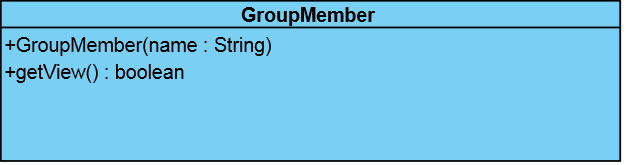
\includegraphics[scale = .5]{res/umlClasses/GroupMember.png}
	\centering
\end{figure}
Das Gruppenmitglied unterscheidet sich vom Gruppenadministrator in sofern, dass ihm die Gruppe betreffend kaum Funktionen zur Verfügung stehen.  
\begin{enumerate}
	\item public GroupMember(name: String)\\
		Konstruktor für einen Gruppenmitglied.
	\item public getView():boolean\\
		Siehe UserDecorator.
\end{enumerate}

\textbf{GoStatus}
\begin{figure}[H]
	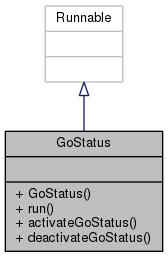
\includegraphics[scale = .5]{res/umlClasses/GoStatus.png}
	\centering
\end{figure}
Der GoStatus bestimmt darüber in welchen Abständen die Position des aktuellen Benutzers an die anderen Gruppenmitglieder übermittelt wird.
\begin{enumerate}
	\item public GoStatus(targetGroupClient: GroupClient)\\
		Konstruktor für den GoStatus wird für jede Gruppe für den aktuellen Benutzer definiert.
	\item public run()\\
		Periodisch bei aktivierten GoStatus der Standort an die Gruppenmitglieder weitergeleitet.
	\item public activateGoStatus()\\
		GoStatus und Gps Tracking aktivieren.
	\item public deactivateGoStatus()\\
		Gps Tracking deaktivieren.
\end{enumerate}

\textbf{Link}
\begin{figure}[H]
	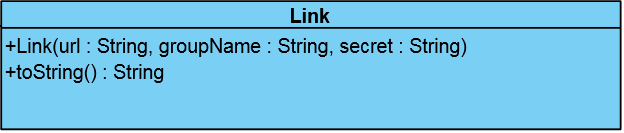
\includegraphics[scale = .5]{res/umlClasses/Link.png}
	\centering
\end{figure}
Mit dem Link kann man andere Mitglieder 
\begin{enumerate}
	\item public Link(url: String, groupName: String , secret: String)\\
		Konstruktor für einen Link. Ein Gruppenlink besteht aus den gelisteten drei Komponenten. Durch den Gruppennamen lässt sich das Mitglied welches den Link betätigt zu derjenigen Gruppe hinzufügen und das sercret verhindert, dass der Link leicht regenerierbar ist.
	\item public toString():String\\
		Der Link wird wieder in seine einzelne Komponenten sortiert.
\end{enumerate}

\textbf{GpsObject}
\begin{figure}[H]
	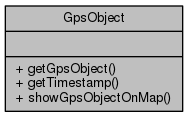
\includegraphics[scale = .5]{res/umlClasses/GpsObject.png}
	\centering
\end{figure}
Das GpsObject gibt an in welcher Form die Gps Daten übermittelt werden.
\begin{enumerate}
	\item public getGpsObject():Point\\
		Der Konstruktor für das GpsObject definiert ein neuen Point der aus einem Längen und einem Breitengrad besteht. 
	\item public getTimestamp():String \\
		Timestamp gibt zurück, wie alt der zuletzt ermittelte Standort ist.
\end{enumerate}

\textbf{Appointment}
\begin{figure}[H]
	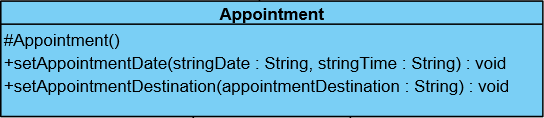
\includegraphics[scale = .6]{res/umlClasses/Appointment.png}
	\centering
\end{figure}
Appointment fasst alle Informationen zusammen die es über den Treffpunkt zu speichern gibt.
\begin{enumerate}
	\item protected Appointment()\\	
		Konstruktor für ein Appointment welches beim Erstellen einer Gruppe default Werte für Datum, Uhrzeit und Ort definiert.
	\item public setAppointmentDate(String stringDate, String stringTime)\\
		Datum und Uhrzeit des Treffens ändern.
	\item getAppointmentDate():AppointmentDate \\
		Datum und Uhrzeit des Appointments zurückgeben.
	\item public setAppointmentDestination(String appointmentDestination)\\
		Über den Namen/Adresse oder über die Position auf der Karte einen Zielort setzen.
	\item public getAppointmentDestination():AppointmentDestination\\
		Den Zielortes des Treffpunktes zurückgeben.
\end{enumerate}

\textbf{AppointmentDate}
\begin{figure}[H]
	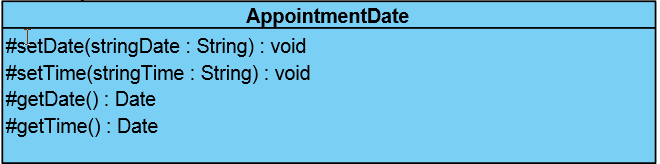
\includegraphics[scale = .5]{res/umlClasses/AppointmentDate.png}
	\centering
\end{figure}
AppointmentDate legt fest wie Datum und Uhrzeit formatiert werden.
\begin{enumerate}
	\item protected setDate(stringDate: String)\\
		Ein Datum festlegen.
	\item protected setTime(stringTime: String)\\
		Eine Uhrzeit festlegen.
	\item protected getDate():Date \\
		Das Datum zurückgeben.
	\item protected getTime():Date \\
		Die Uhrzeit zurückgeben.
\end{enumerate}

\textbf{AppointmentDestination}
\begin{figure}[H]
	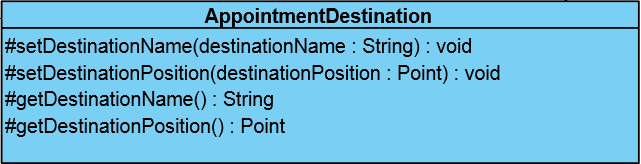
\includegraphics[scale = .5]{res/umlClasses/AppointmentDestination.png}
	\centering
\end{figure}
AppointmentDestination legt fest wie Name und Position des Zielortes definiert sind.
\begin{enumerate}
	\item protected setDestinationName(destinationName:String)\\
		Den Zielort über den Namen/ die Adresse bestimmen.
	\item protected setDestinationPosition(destinationPosition:Point)\\
		Den Zielort über eine Position auf der Karte bestimmen.
	\item protected getDestinationName():String \\
		Den Zielortnamen zurückgeben.
	\item protected getDestinationPosition():Point \\
		Die Zielortposition zurückgeben.
\end{enumerate}

